\documentclass[report,12pt]{article}
\usepackage{graphicx}
\usepackage{hyperref}
\usepackage{longtable}
\hypersetup{
    colorlinks=true,
    linkcolor=red,      
    urlcolor=blue,
    citecolor=green     
}

\title{\textbf{Reporte de Pruebas Exploratorias}}
\author{Andres Gomez, Natalia Hernandez, Ramon Espinosa, Stiven Cardona}
\date{\today}

\begin{document}

\maketitle

\section{Introducción}
El objetivo de estas pruebas exploratorias es evaluar la estabilidad, facilidad de uso y comportamiento de Ghost CMS en diferentes escenarios, explorando su editor, administración de contenido y configuraciones.

\section{Sistema de registro de incidencias}
Para el registro de incidencias se escogio usar github issues dado que:
\begin{enumerate}
    \item \textbf{Integración Nativa con el Repositorio:} GitHub Issues se encuentra integrado directamente en el repositorio del proyecto que creamos para el equipo.
    \item \textbf{Seguimiento y Organización Eficiente:} Ofrece etiquetas, hitos y proyectos tipo Kanban que permiten clasificar y priorizar incidencias de manera organizada.
    \item \textbf{Colaboración Transparente:} GitHub Issues permite la participación de todo el equipo y de los profesores y tutores asignados para la revision. Los comentarios y menciones facilitan la comunicación y el seguimiento de cada incidencia en un solo lugar.
\end{enumerate}

\href{https://github.com/stivencardonauniandes/pruebas-automatizadas/issues}{Enlace de acceso al sistema de registro de incidencias}

\section{Listado de funcionalidades identificadas}
En esta sección del reporte de pruebas exploratorias, se documentan las funcionalidades clave exploradas durante las sesiones de prueba. Se describe cada funcionalidad evaluada, destacando su propósito dentro del sistema y cualquier comportamiento relevante observado se podra evidenciar en el apartado de escenarios de prueba.

\begin{longtable}{|p{0.5cm}|p{1.5cm}|p{2cm}|p{6.5cm}|p{3cm}|}
    \hline
    \textbf{\#} & \textbf{Modulo} & \textbf{Nombre} & \textbf{Descripción} & \textbf{Autor} \\
    \hline
    1 & Pages & New page & Permite al usuario crear una nueva pagina, la cual permite agregar multiples elementos como textos, videos, imagenes, codigo, botones y muchos mas & Andres Gomez \\
    \hline
    2 & Posts & New post & Permite al usuario previamente identificado como administrador crear un nuevo post al blog de la aplicacion web & Stiven Cardona \\
    \hline
    3 & Posts & List posts & Al ingresar a la seccion posts del administrador permite al usuario visualizar todos los posts que se han creado y ordernarlos de acuerdo a diferentes criterios & Stiven Cardona \\
    \hline
    4 & Posts & Publish post & Permite al usuario publicar un post que ha sido creado/editado previamente en la pagina web & Stiven Cardona \\
    \hline
    5 & Pages & Edit page & Permite al usuario editar una pagina ya creada, la cual permite al igual que crear una pagina agregar multiples elementos como textos, videos, imagenes, codigo, botones y muchos mas & Andres Gomez \\
    \hline
    6 & Pages & Publish page & Permite al sistema publicar paginas, esta dispone de un link en la cual se puede entrar desde cualquier navegador & Andres Gomez \\
    \hline
    7 & Pages & List pages & Permite al usuario ver todas las paginas creadas, mostrando informacion como Titulo, Creado Por, Utilma fecha de modificacion y si esta publicada o esta en estado Draft & Andres Gomez \\
    \hline
    8 & Tags & Create tag & Permite al usuario crear un tag a partir de hacer click en el boton "new tag" ubicado en la parte superior derecha en la pagina de Tags, directamente al crear un post en settings , requiriendo especificar un name de forma obligatoria. Si el name tiene caracter \#, es un Internal tag, sino es Publico. Otros atributos opcionales son color, slug, descripcion de 500 caracteres maximo e image & Natalia Hernandez \\
    \hline
    9 & Tags & View tag & Permite al usuario una vez creado un tag, en la opcion de edicion de ese tag, la opcion de ver todos los post asociados a ese tag con el boton "view" ubicado en la parte superior derecha. & Natalia Hernandez \\
    \hline
    10 & Tags & List tags & Permite al usuario  listar todos los tags que ha creado en la barra superior izquierda opcion tags, filtrando por Public e Internal tags, a su vez, se muestra el numero de post asociados. Al hacer click en el tag, se abre la opcion editar tag & Natalia Hernandez \\
    \hline
    11 & Tags & Edit tag & Permite al usuario editar un post ya creado en el blog de la aplicacion web. El usuario puede modificar todos los atributos, requiriendo especificar un name de forma obligatoria. Si el name tiene caracter \#, es un Internal tag, sino es Publico. Otros atributos opcionales son color, slug, descripcion de 500 maximo e image & Natalia Hernandez \\
    \hline
    12 & Tags & Delete tag & Permite al usuario borrar el tag al darle click al boton  rojo "Delete tag" ubicado en la parte inferior izquierda. Al darle click, se abre un mensaje de confirmacion con la opcion Cancel y Delete & Natalia Hernandez \\
    \hline
    13 & Posts & Edit posts & Permite al usuario editar un post ya creado en el blog de la aplicacion web si el mismo esta en modo draft. & Stiven Cardona \\
    \hline
    14 & Members & Create member & Permite al usuario crear un nuevo miembro del sitio. Esto para poder condicionar el acceso al contenido del sitio & Ramon Espinosa \\
    \hline
    15 & Members & List members & Permite al usuario listar todos los miembros que están suscritos al sitio y el contenido que se distribuye a su nombre & Ramon Espinosa \\
    \hline
    16 & Members & Edit members & Permite al usuario editar los atributos asociados a un miembro como nombre, correo, notas y si se quiere enviar notificaciones al miebro via correo electrónico & Ramon Espinosa \\
    \hline
    17 & Members & Import members & Permite crear miembros en masa importando la lista de miembros que se quieren crear de un archivo csv & Ramon Espinosa \\
    \hline
\end{longtable}

\href{https://docs.google.com/spreadsheets/d/1AW5Uuod1t0fUaCuIDGt3VsMxNsfL1ElC/edit?usp=sharing&ouid=113118362463883688087&rtpof=true&sd=true}{Enlace al archivo en formato .xlsx}

\section{Inventario de pruebas}
\begin{enumerate}
    \item Escenario de pruebas exploratorias \textbf{Andres Gomez}
    \begin{itemize}
        \item \textbf{Aplicación bajo prueba:} Ghost
        \item \textbf{Versión/Hash commit:} 5.114.1 - SHA f890beda35ddb56e4fcdbad1a7c190c3e5728d79
        \item \textbf{Ambiente de pruebas:} Brave Version: 1.76.80 , Windows 10 64Bits 1861 x 848
        \item \textbf{Tester:} Andres Gomez
        \item \textbf{Enlace del reporte:} \href{https://docs.google.com/spreadsheets/d/1AW5Uuod1t0fUaCuIDGt3VsMxNsfL1ElC/edit?gid=2070240166#gid=2070240166}{https://docs.google.com/spreadsheets/andres-gomez}
    \end{itemize}
    \item Escenario de pruebas exploratorias \textbf{Natalia Hernandez}
    \begin{itemize}
        \item \textbf{Aplicación bajo prueba:} Ghost
        \item \textbf{Versión/Hash commit:} 5.114.1 - SHA f890beda35ddb56e4fcdbad1a7c190c3e5728d79
        \item \textbf{Ambiente de pruebas:} Firefox Version: 136.0.3 , Windows 11 64Bits
        \item \textbf{Tester:} Natalia Hernandez
        \item \textbf{Enlace del reporte:} \href{https://docs.google.com/spreadsheets/d/1AW5Uuod1t0fUaCuIDGt3VsMxNsfL1ElC/edit?gid=978517391#gid=978517391}{https://docs.google.com/spreadsheets/natalia-hernandez}
    \end{itemize}
    \item Escenario de pruebas exploratorias \textbf{Ramon Espinosa}
    \begin{itemize}
        \item \textbf{Aplicación bajo prueba:} Ghost
        \item \textbf{Versión/Hash commit:} 5.114.1 - SHA f890beda35ddb56e4fcdbad1a7c190c3e5728d79
        \item \textbf{Ambiente de pruebas:} Google Chrome Version: 134.0.6998.177 (Official Build) (64-bit), Windows 11 64Bits
        \item \textbf{Tester:} Ramon Espinosa
        \item \textbf{Enlace del reporte:} \href{https://docs.google.com/spreadsheets/d/1AW5Uuod1t0fUaCuIDGt3VsMxNsfL1ElC/edit?gid=820482743#gid=820482743}{https://docs.google.com/spreadsheets/ramon-espinosa}
    \end{itemize}
    \item Escenario de pruebas exploratorias \textbf{Stiven Cardona}
    \begin{itemize}
        \item \textbf{Aplicación bajo prueba:} Ghost
        \item \textbf{Versión/Hash commit:} 5.114.1 - SHA f890beda35ddb56e4fcdbad1a7c190c3e5728d79
        \item \textbf{Ambiente de pruebas:} Safari Version: 17.4, MacOS Sonoma 14.7.4
        \item \textbf{Tester:} Stiven Cardona
        \item \textbf{Enlace del reporte:} \href{https://docs.google.com/spreadsheets/d/1AW5Uuod1t0fUaCuIDGt3VsMxNsfL1ElC/edit?gid=1462193001#gid=1462193001}{https://docs.google.com/spreadsheets/stiven-cardona}
    \end{itemize}
\end{enumerate}

\section{Modelo GUI}
En este modelo describimos cómo los usuarios interactúan con la interfaz gráfica de Ghost y cómo se relacionan las distintas pantallas o módulos a través de transiciones.\\

A continuación adjuntamos un enlace al modelo GUI construido usando la herramienta draw.io, \href{https://drive.google.com/file/d/1O5UubtcBZ5smm2bCaAbsnGFKy3dRc_7O/view?usp=sharing}{enlace al modelo GUI del CMS Ghost}\\


\textbf{Nota:} Para interactuar con el modelo se debe seleccionar la opcion para abrir el enlace con la plataforma con draw.io, a traves de google drive\\

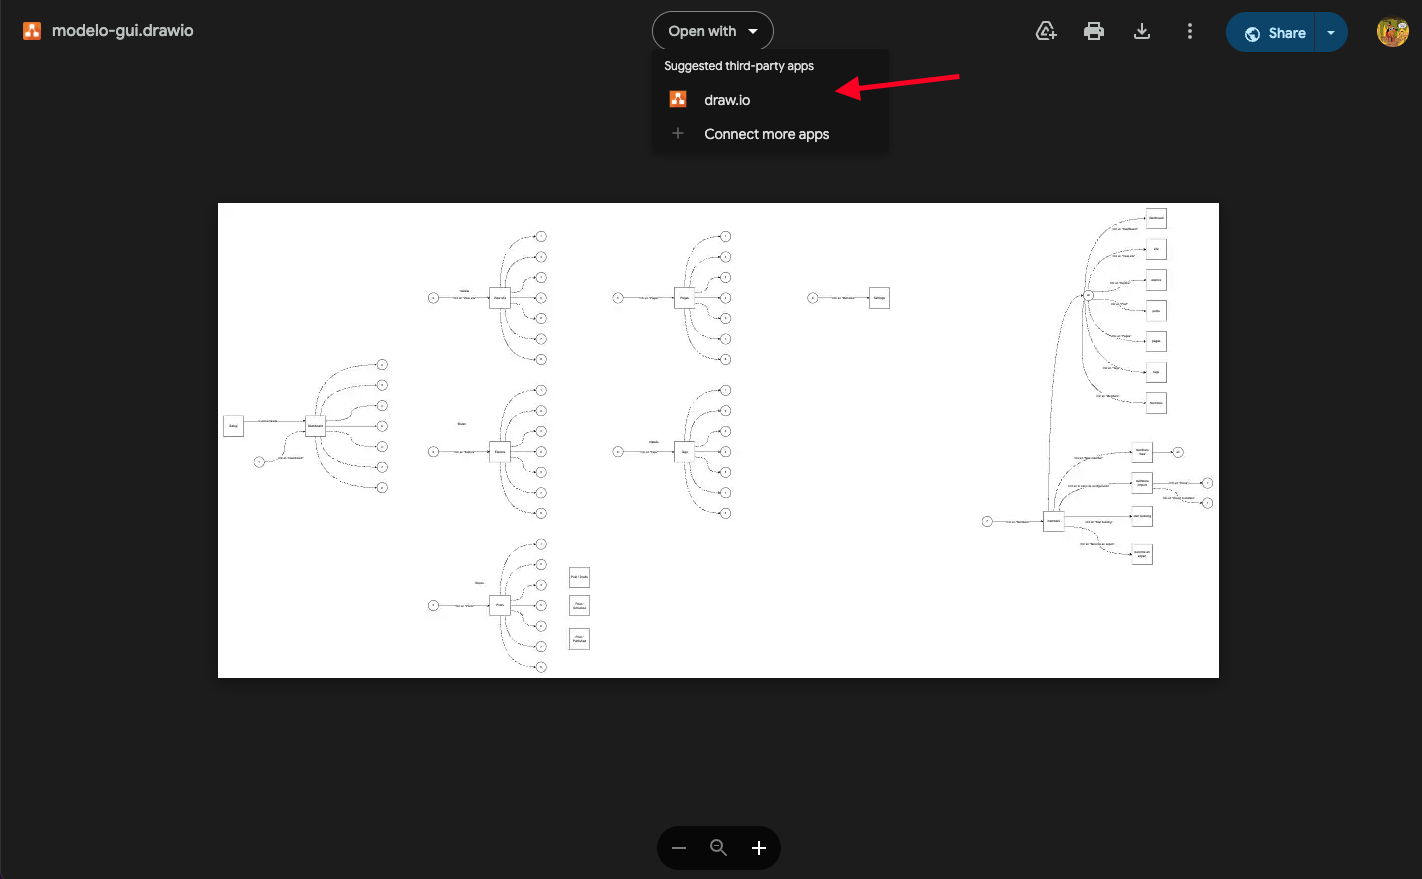
\includegraphics[width=1\linewidth]{image.png}

\section{Modelo de dominio}
En este modelo describimos las entidades, atributos y  tipos de datos que se manejan en  el CMS Ghost, decidimos usar un diagrama de clases con notacion UML a traves de la herramienta draw.io, \href{https://drive.google.com/file/d/1AeHiRqBHY_PK6NRBMy1sDqH8jC6v0vbe/view?usp=sharing}{enlace al modelo de dominio del CMS Ghost}
\end{document}
